%==================================================
%      PREAMBOLO e DICHIARAZIONI INIZIALI
%==================================================
\documentclass[10pt,oneside,a4paper]{article}

\usepackage[latin1]{inputenc} 
\usepackage[italian]{babel}
\usepackage[T1]{fontenc}
\usepackage{siunitx} %Inserisce automaticamente i dati con le unit�  di misura correttamente formattate del SI (utilizzo: \SI{0.82}{m^2}, in generale \SI{misura con il punto decimale}{unit�  di misura})
\sisetup{output-decimal-marker = {.}, separate-uncertainty = true, input-uncertainty-signs = \pm, detect-weight=true, detect-family=true} %per usare SI con il punto decimale
\usepackage{listings} %Per citare codice informatico formattandolo correttamente
\usepackage{amsmath,amsthm,verbatim,amssymb,amsfonts,amscd,graphicx,mathtools}
\usepackage[makeroom]{cancel}
\newcommand{\abs}[1]{\left\lvert\,#1\,\right\rvert}
\usepackage{geometry}
\usepackage{epigraph}
\usepackage{booktabs}	%tabelle migliorate
\usepackage{tablefootnote}	%note a pi� di pagina in tabella
\usepackage{threeparttable} %tabella con note a pi� di tabella
\usepackage{caption}	%descrizione per figure
\usepackage{dblfnote}
\captionsetup{tableposition=top,figureposition=bottom,font=small} %setup descrizione
\usepackage{float}
\usepackage{esvect} %vettori
\usepackage{longtable} %tabelle lunghe
\usepackage[dvipsnames]{xcolor}
\definecolor{sepia}{HTML}{80002A}
\usepackage[colorlinks=true, citecolor=black, linkcolor=sepia, urlcolor=black]{hyperref}
\usepackage{mathrsfs}
\usepackage{circuitikz}


\usepackage{multicol}
\newenvironment{Figure}
  {\par\medskip\noindent\minipage{\linewidth}}
  {\endminipage\par\medskip}

\newcommand{\var}{\operatorname{var}}
\newcommand{\cov}{\operatorname{cov}}


\usepackage{listings} %Per inserire codice
\lstnewenvironment{codice_c}[1][]
{\lstset{basicstyle=\small\ttfamily, columns=fullflexible,
keywordstyle=\color{red}\bfseries, commentstyle=\color{blue},
language=C, basicstyle=\small,
numbers=left, numberstyle=\tiny,
stepnumber=2, numbersep=5pt, frame=shadowbox,  showstringspaces=false, #1}}{}

%==================================================
%                  PRIMA PAGINA
%==================================================

\title{\textsc{\textbf{Esercitazione 4}: Amplificatore operazionale 2}}
\author{\small{G. Galbato Muscio} \and \small{L. Gravina} \and \small{L. Graziotto}}
\date{6 Novembre 2018}

\begin{document}
	\begin{figure}
		\centering
		
\includegraphics[scale=0.5, trim={2.8cm 8.9cm 0 9cm}, clip]{logo.png}
	\end{figure}
	\maketitle
	\begin{center} 
		\fbox{{\fontsize{12pt}{8mm}\textsc{Gruppo 11}}} \\
	\end{center}
\hrule
\vspace{0.5cm}
\renewcommand{\abstractname}{Abstract}
\begin{abstract}
Si realizzano un amplificatore differenziale e un sommatore non invertente utilizzando l'amplificatore operazionale LM358N. Si misurano le amplificazioni comune e differenziale e il CMRR a diverse frequenze.
\end{abstract}
\vspace{4cm}
\tableofcontents %Indice
\newpage


\pagebreak
\begin{multicols}{2}
%==================================================
%      		AMPLIFICATORE DIFFERENZIALE
%==================================================
\section{Amplificatore differenziale}
Si utilizza nel seguito l'amplificatore operazionale LM358N, e lo si alimenta con una differenza di potenziale di $\pm \SI{15}{V}$, connettendo gli ingressi \texttt{V+} e \texttt{GND} alla doppia alimentazione in continua, positiva e negativa. 

Si realizza un amplificatore differenziale con guadagno $G = 5$, come nel circuito seguente.

\begin{center}
\begin{circuitikz}
\draw (0,0) node[op amp] (opamp) {}
(opamp.+) to[R=$R_1'$] ++(-2,0) node[circ] {} node[left] {$v_\text{2}$}
(opamp.-) to[short] ++(0, 1.25) to[R = $R_2$] ++(2,0) -| (opamp.out)
(opamp.-) node[circ] {}
(opamp.+) node[circ] {}
(opamp.-) to[R=$R_1$] ++(-2,0) node[circ] {} node[left] {$v_1$}
(opamp.out) to[short, *-*] ++(0.5,0) node[right] {$v_\text{o}$}
(opamp.+) to[R=$R_2'$] ++(0,-2) node[ground] {}
;\end{circuitikz}
\end{center}

Scegliendo $R_1 = R_1'$ e $R_2 = R_2'$ si ha la relazione 
\[
v_o = \frac{R_2}{R_1}(v_2-v_1),
\]
ovvero il segnale in uscita � proporzionale alla differenza tra i segnali in ingresso. Pertanto si costruir� un circuito in cui i valori di $R_1$ e $R_1'$ e di $R_2$ e $R_2'$ siano il pi� simili possibile, e si sceglier� $R_2 / R_1 =: G = 5$. Per ottenere questo scopo, si utilizzeranno dei resistori per $R_1$ e $R_2$, e dei trimmer per $R_1'$ e $R_2'$, la cui resistenza � regolabile con pi� finezza mediante un cacciavite.

Le resistenze utilizzate, misurate con il multimetro, sono
\[
\begin{aligned}
R_1 &= \SI{4.64 \pm 0.02}{k\ohm} \\
R_1' &= \SI{4.64 \pm 0.02}{k\ohm} \\
R_2 &= \SI{21.8 \pm 0.1}{k\ohm} \\
R_2' &= \SI{21.7 \pm 0.1}{k\ohm}.
\end{aligned}
\]

Si misurano quindi l'amplificazione di modo comune $A_c$ e l'amplificazione differenziale $A_d$, nonch� il Common Mode Rejection Ratio (CMRR), $\rho = \abs{A_d / A_c}$, e li si confronta con i loro valori attesi dati i componenti del circuito e con quelli caratteristici di un amplificatore differenziale ideale.

Per misurare $A_c$ si invia lo stesso segnale ai due ingressi, ossia un segnale sinusoidale di frequenza $f$ e ampiezza $V_i$, che � abbastanza grande per osservare l'attenuazione data dal piccolo valore di $A_c$ e minore di \SI{10}{V} (si veda l'istantanea dell'oscilloscopio in figura~\ref{fig:Ac_differenziale}), valore oltre il quale si osservano distorsioni. Si riportano in tabella~\ref{tab:Ac_differenziale} le misure compiute a diverse frequenze. Il valor medio con associata la deviazione standard �
\[
A_c = \SI{3.01 \pm 0.08 e-3}{}.
\]

\begin{Figure}
	\begin{center}
	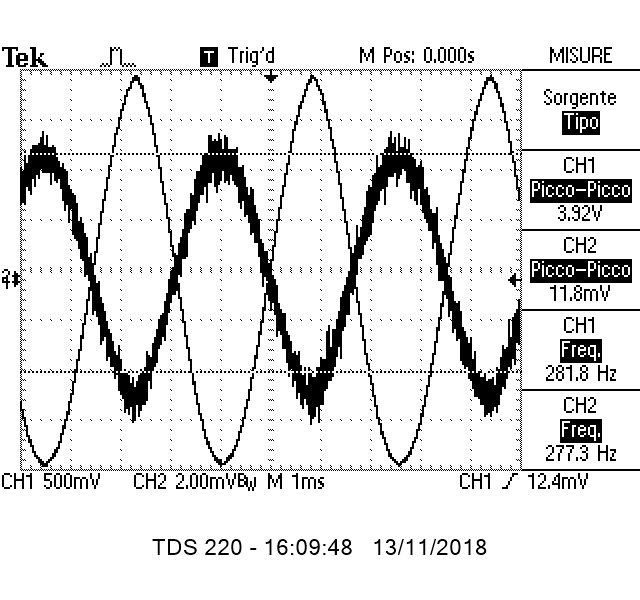
\includegraphics[width=\linewidth]{comune.png}
	\captionof{figure}{Istantanea dell'oscilloscopio per l'amplificatore differenziale, misura di $A_c$}
	\label{fig:Ac_differenziale}
	\end{center}
\end{Figure}

\begin{center}
\captionof{table}{Misure per la stima di $A_c$}
\label{tab:Ac_differenziale}
\begin{tabular}{c|c|c|c}
$f$ [\SI{}{Hz}] & $V_i$ [\SI{}{V}] & $v_o$ [\SI{}{mV}] & $A_c = v_o / V_i$ \\
\hline
      149.5 &        3.90 &         11.3 & 2.90e-03 \\
      222.0 &        3.90 &         11.5 & 2.95e-03 \\
      281.0 &        3.90 &         11.8 & 3.03e-03 \\
      359.0 &        3.90 &         11.8 & 3.03e-03 \\
      461.0 &        3.90 &         12.2 & 3.13e-03 \\
\hline
\end{tabular}
\end{center}

Per misurare $A_d$ si devono invece ricavare singolarmente le amplificazioni $A_1$ e $A_2$, inviando un solo segnale ad un ingresso e mettendo a terra l'altro. Inviando il segnale a $v_1$ e mettendo a terra $v_2$ si avr� un amplificatore invertente, dunque ci si aspetta di ottenere 
\[
A_1 = -\frac{R_2}{R_1}.
\]
Inviando il segnale a $v_2$ e mettendo a terra $v_1$, invece, si avr� un amplificatore non invertente, dunque ci si aspetta di ottenere 
\[
A_2 = \frac{R_2'}{R_1}\frac{R_1+R_2}{R_1'+R_2'}.
\] 

Si invia dunque alternativamente ad un ingresso e poi all'altro (mettendo a terra quello non usato) un segnale sinusoidale di ampiezza $v_{1,2}$ e frequenza $f$, e si misura l'uscita $v_o$ sul canale \texttt{CH2} dell'oscilloscopio. Per l'amplificatore invertente si osserva correttamente lo sfasamento di $\pi$ tra ingresso e uscita, come visibile nello screenshot di figura~\ref{fig:invertente_differenziale}. Quindi si ricavano $A_1 = v_o / v_1$ e $A_2 = v_o / v_2$ e l'amplificazione differenziale $A_d = (A_1 - A_2) / 2$. Si riportano in tabella~\ref{tab:Ad_differenziale} le misure compiute a diverse frequenze.

\begin{Figure}
	\begin{center}
	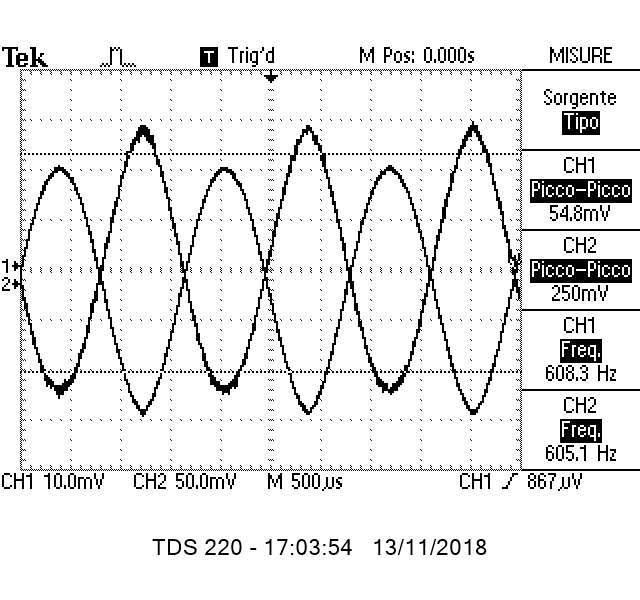
\includegraphics[width=\linewidth]{differenziale.png}
	\captionof{figure}{Istantanea dell'oscilloscopio per l'amplificatore differenziale, ingresso invertente}
	\label{fig:invertente_differenziale}
	\end{center}
\end{Figure}

\begin{table*}
\begin{center}
\captionof{table}{Misure per la stima di $A_d$, si riporta anche il valore della tensione in ingresso $v_o$ in quanto si � osservato che questa cambiava passando da un'ingresso ad un altro}
\label{tab:Ad_differenziale}
\begin{tabular}{c|c|c|c|c|c|c|c}
$f$ [\SI{}{kHz}] & $v_1$ ($v_2 = 0$) [\SI{}{mV}] & $v_o$ ($v_2 = 0$) [\SI{}{mV}] & $v_2$ ($v_1 = 0$) [\SI{}{mV}] & $v_o$ ($v_1 = 0$) [\SI{}{mV}] & $A_1$ & $A_2$ & $A_d$\\
\hline
      111.4 &             54.5 &           -250.0 &             54.8 &            250.0 &   -4.59 &    4.56 &   -4.57 \\
      210.0 &             54.8 &           -248.0 &             55.6 &            250.0 &   -4.53 &    4.50 &   -4.51 \\
      282.0 &             54.8 &           -248.0 &             55.0 &            250.0 &   -4.53 &    4.55 &   -4.54 \\
      303.0 &             55.0 &           -250.0 &             55.4 &            250.0 &   -4.55 &    4.51 &   -4.53 \\
      363.0 &             54.4 &           -250.0 &             55.4 &            250.0 &   -4.60 &    4.51 &   -4.55 \\
      398.0 &             54.8 &           -249.0 &             55.6 &            250.0 &   -4.54 &    4.50 &   -4.52 \\
      460.0 &             55.0 &           -250.0 &             55.2 &            251.0 &   -4.55 &    4.55 &   -4.55 \\
      605.0 &             54.8 &           -249.0 &             55.4 &            250.0 &   -4.54 &    4.51 &   -4.53 \\
\hline
\end{tabular}
\end{center}
\end{table*}

Si hanno come valori medi delle amplificazioni di singolo canale 
\[
\begin{aligned}
A_1 &= -4.55 \pm 0.02 \\
A_2 &= 4.52 \pm 0.02
\end{aligned}
\]
compatibili con i valori attesi dati i componenti usati 
\[
\begin{aligned}
A_1^\text{\tiny{(atteso)}} &= -4.70 \pm 0.05 \\
A_2^\text{\tiny{(atteso)}} &= 4.70 \pm 0.05.
\end{aligned}
\]
Il valore medio dell'amplificazione differenziale, con associata incertezza data dalla deviazione standard, �
\[
A_d = -4.53 \pm 0.05,
\]
compatibile con il valore atteso dati i componenti di $A_d^\text{\tiny{(atteso)}} = -4.69 \pm 0.05$. Si pu� confrontare anche il valore misurato di $A_c$ con quello atteso $A_c^\text{\tiny{(atteso)}} = A_1 + A_2 = -0.004 \pm 0.010$, osservando che essi sono compatibili; si sottolinea che l'errore sul valore previsto di $A_c$ � relativamente ingente proprio perch� ottenuto da una differenza di grandezze i cui valori sono quasi uguali.

Si nota inoltre che il valore di $A_c$ � prossimo allo zero, mentre quello di $A_d$ al valore pari al guadagno $G = 5$, secondo il quale sono state scelte le resistenze all'inizio.

Si stima quindi il CMRR 
\[
\rho = \abs{\frac{A_d}{A_c}} = \SI{1.51 \pm 0.06 e3}{},
\]
compatibile con il valore atteso di $\rho \simeq \SI{1.2 e3}{}$, che � fornito qui senza incertezza in quanto essa non � stimabile, dal momento che l'errore relativo sul valore atteso di $A_c$ � maggiore del $200\%$, come visto prima. Si osserva che questo valore � dello stesso ordine di grandezza di quello riportato nel datasheet, ossia $\rho = 65 \div 80 \SI{}{dB}$; nell'amplificatore differenziale ideale, invece, si dovrebbe avere $\rho \rightarrow \infty$.

%==================================================
%    		SOMMATORE NON INVERTENTE
%==================================================
\section{Sommatore non invertente}
Si realizza un circuito sommatore non invertente a due ingressi, come indicato nella figura seguente.

\begin{center}
\begin{circuitikz}
\draw (0,0) node[op amp] (opamp) {}
(opamp.out) to[short, *-*] ++(0.5,0) node[right] {$V_\text{o}$}
(opamp.-) to[short] ++(-0.25,0) to[R=$R$] ++(-1.5,0) node[ground] {}
(opamp.-) -| ++(0,1) to[R = $R'$] ++(2,0) -| (opamp.out)
(opamp.-) node[circ] {}
(opamp.+) to[R=$R_A$] ++(-2,0) node[circ] {} node[left]{$V_A$}
(opamp.+) node[circ] {}
(opamp.+) to[short] ++(0,-1) to[R=$R_B$] ++(-2,0) node[circ] {} node[left]{$V_B$}
;\end{circuitikz}
\end{center}

I valori delle resistenze utilizzate, misurati con il multimetro, sono
\[
\begin{aligned}
R_A &= \SI{8.11 \pm 0.04}{k\ohm} \\
R_B &= \SI{8.13 \pm 0.04}{k\ohm} \\
R &= \SI{8.10 \pm 0.04}{k\ohm} \\
R' &= \SI{8.11 \pm 0.04}{k\ohm}; 
\end{aligned}
\]

Anche in questo caso, per avere resistenze simili tra loro, in modo che valga la relazione
\[
V_o = \frac{R'+R}{R} \frac{R}{2} \left[\frac{V_A}{R_A} + \frac{V_B}{R_B} \right] \simeq V_A + V_B,
\]
si sono utilizzati un resistore per $R'$ e dei trimmer per $R$, $R_A$ ed $R_B$.

Si ha cura di rispettare la disuguaglianza $V_o^\text{max} < \SI{15}{V}$ per mantenere l'amplificatore nella regione di lavoro, in quanto esso � alimentato, come nella sezione precedente, con una tensione di $\pm \SI{15}{V}$.

Si misurano le amplificazioni dei singoli ingressi, inviando un segnale sinusoidale di frequenza $f$ e ampiezza $V_{A,B}$ alternativamente all'ingresso $A$ o $B$ e mettendo a terra l'ingresso non utilizzato. Si riportano in tabella~\ref{tab:AB_noninvertente} le misure a diverse frequenze.

\begin{table*}
\begin{center}
\captionof{table}{Misure delle singole amplificazioni per il sommatore non invertente}
\label{tab:AB_noninvertente}
\begin{tabular}{c|c|c|c|c|c}
$f$ [\SI{}{kHz}] & $V_{A,B}$ [\SI{}{V}] & $V_o$ (con $V_B = 0$) [\SI{}{V}] & $V_o$ (con $V_A = 0$) [\SI{}{V}] & $A_A$ & $A_B$ \\
\hline
        277 &        3.82 &            3.84 &            3.84 &    1.01 &    1.01 \\
        534 &        3.84 &            3.84 &            3.84 &    1.00 &    1.00 \\
       1047 &        3.84 &            3.84 &            3.84 &    1.00 &    1.00 \\
\hline
\end{tabular}
\end{center}
\end{table*}

Otteniamo quindi come valori medi delle singole amplificazioni
\[
\begin{aligned}
A_A &= 1.00 \pm 0.03 \\
A_B &= 1.00 \pm 0.03,
\end{aligned}
\]
compatibili con i valori previsti, dati i componenti utilizzati, di
\[
\begin{aligned}
A_A^\text{\tiny{(atteso)}} &= \frac{R_B}{R_A + R_B} \frac{R' + R}{R} = 1.00 \pm 0.01 \\
A_B^\text{\tiny{(atteso)}} &= \frac{R_A}{R_A + R_B} \frac{R' + R}{R} = 1.00 \pm 0.01.
\end{aligned}
\]

Verifichiamo il comportamento del circuito inviando un segnale sinusoidale di frequenza $f = \SI{21.2 \pm 0.6}{kHz}$ e ampiezza picco-picco $V_\text{in} = \SI{2.28 \pm 0.07}{V}$ all'ingresso $A$ e un segnale continuo di \SI{5.00 \pm 0.03}{V}, ricavato dall'alimentatore, all'ingresso $B$. Si riporta in figura~\ref{fig:continua_sinusoidale} uno screenshot dell'oscilloscopio per questa configurazione: si osserva come il segnale sinusoidale sia traslato verso l'alto\footnote{� bene notare che i \emph{ground} dei due canali sono allineati e che le scale di tensione sono coerenti.}.

\begin{Figure}
	\begin{center}
	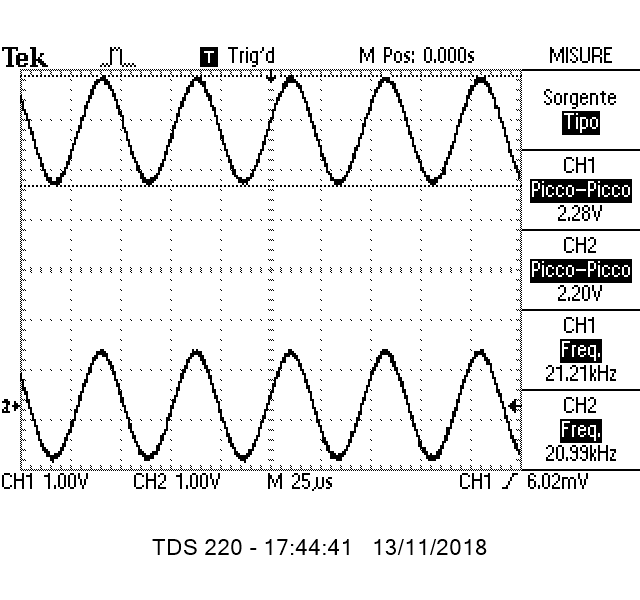
\includegraphics[width=\linewidth]{shift.png}
	\captionof{figure}{Istantanea dell'oscilloscopio in cui � visibile la somma di una sinusoide (in basso) con un segnale in continua di \SI{5}{V}}
	\label{fig:continua_sinusoidale}
	\end{center}
\end{Figure}

Si inviano dunque ai due ingressi due segnali sinusoidali di medesima ampiezza $V_\text{in} = \SI{848 \pm 25}{mV}$ e frequenze rispettivamente di $f_1 = \SI{1.15 \pm 0.03}{kHz}$ e $f_2 = \SI{1.09 \pm 0.03}{kHz}$; si osserva in uscita il fenomeno dei battimenti, ovvero si ha una $V_o$ sinusoidale la cui ampiezza varia seguendo una sinusoide di frequenza minore.

Si pu� stimare la frequenza dell'inviluppo con i cursori (e avendo cura di impostare la modalit� singola del \texttt{TRIGGER}), ottenendo $f_\text{inv} = \SI{28.3 \pm 0.8}{Hz}$; si confronta questo valore con quello previsto di 
\[
f_\text{inv}^\text{\tiny{(atteso)}} = \frac{f_1 - f_2}{2} = \SI{30 \pm 2}{Hz}, 
\]
e si osserva che sono compatibili. Si riporta in figura~\ref{fig:battimenti_ingresso} lo screenshot per i due segnali in ingresso: si nota che essi hanno frequenza di poco differente, osservando lo sfasamento progressivo lungo la schermata dei massimi. 

\begin{Figure}
	\begin{center}
	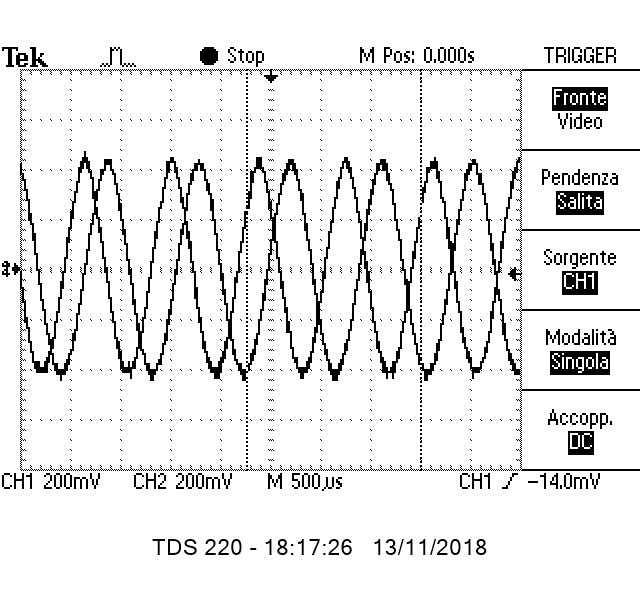
\includegraphics[width=\linewidth]{battimentiIngresso.png}
	\captionof{figure}{Istantanea dell'oscilloscopio per il fenomeno dei battimenti, segnali in ingresso}
	\label{fig:battimenti_ingresso}
	\end{center}
\end{Figure}

\begin{Figure}
	\begin{center}
	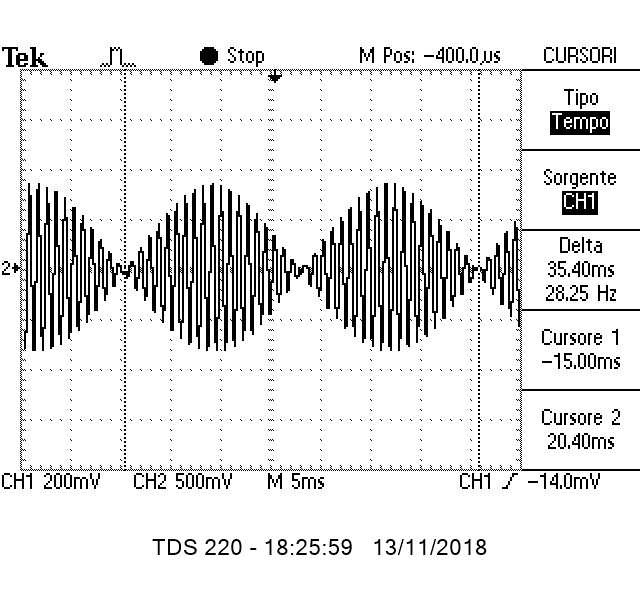
\includegraphics[width=\linewidth]{battimenti5.png}
	\captionof{figure}{Istantanea dell'oscilloscopio per il fenomeno dei battimenti, segnale in uscita}
	\label{fig:battimenti_uscita}
	\end{center}
\end{Figure}

Si riporta invece in figura~\ref{fig:battimenti_uscita} lo screenshot del segnale in uscita: � evidente l'inviluppo dei due, che procede alla frequenza $f_\text{inv}$ stimata precedentemente.

\begin{Figure}
	\begin{center}
	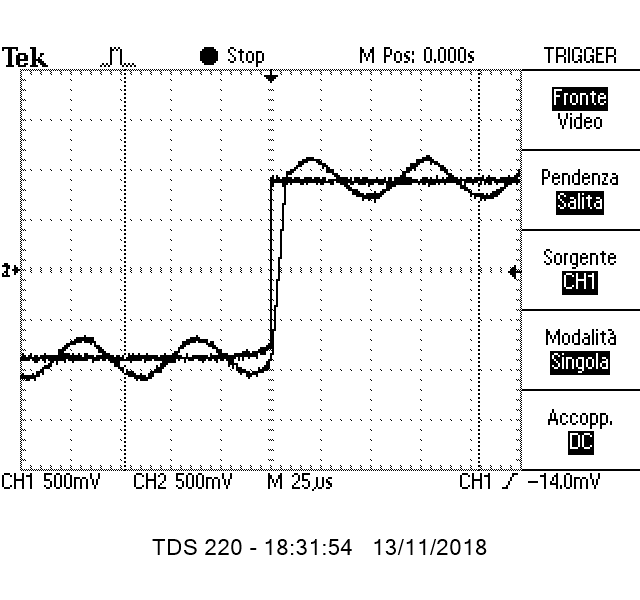
\includegraphics[width=\linewidth]{quadraSinusoide.png}
	\captionof{figure}{Istantanea dell'oscilloscopio per la somma di sinusoide e onda quadra}
	\label{fig:quadra_seno}
	\end{center}
\end{Figure}

Infine si invia un segnale sinusoidale di frequenza $f = \SI{17.4 \pm 0.5}{kHz}$ e di ampiezza picco-picco $V_\text{in} = \SI{392 \pm 12}{mV}$ all'ingresso $B$ e un'onda quadra di frequenza inferiore a quella della sinusoide, $f = \SI{277 \pm 8}{Hz}$, e ampiezza picco-picco $V = \SI{1.82 \pm 0.05}{V}$ all'ingresso $A$. Si riporta in figura~\ref{fig:quadra_seno} l'istantanea dell'oscilloscopio per il segnale di uscita, e si osserva come la sinusoide segua l'andamento dell'onda quadra. 




\end{multicols}
\end{document}